\documentclass[10pt,a4paper]{book}
\usepackage[utf8]{inputenc}
\usepackage{amsmath}
\usepackage{amsthm}
\usepackage{amsfonts}
\usepackage{amssymb}
\usepackage{geometry}
\usepackage{graphicx}
\usepackage{enumitem}
\author{Nicolò Fornari}
\title{Network security}
\newtheorem{remark}{Remark}
\begin{document}
\maketitle
\chapter{Network protocols}
\section{Introduction}
\textbf{Data link layer}\\
It is the lowest logical level, the data link interconnects physical interfaces. Each interface is identified by a MAC address (Media Access Control).\\
The MAC address is 48 bit long, it is usually represented in Hex notation and it is used to route packets in local networks.\\
It uniquely identifies a network interface. It is assigned by the producer according to the standard IEEE 802.\\\\
\textbf{Network Layer}\\
IP operates at this level. IP addresses are dynamically assigned by an authority (eg. ISP's DHCP server).\\\\
\textbf{Stateful:} communication starts, develops,ends. eg. TCP\\
\textbf{Stateless:} IP\\
\newpage
\section{ARP}
ARP (address resolution protocol) allows systems to associate an ip address to a MAC address.\\
All addresses in the ARP table are added by one of these mechanisms:
\begin{itemize}
\item ARP request-reply: \\
who is 192.168.0.16 tell 192.168.0.1\\
192.168.0.16 is at 00-10-BC-2c-11-56
\item Gratuitous ARP\\
192.168.0.16 is at 00-10-BC-2c-11-56
\end{itemize}
\textbf{ARP frame header}\\\\
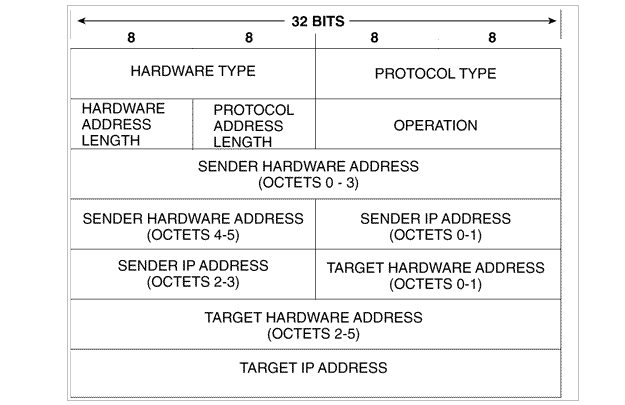
\includegraphics[scale=0.6]{arp.png}\\
\textbf{ARP poisoning}\\
The ARP protocol is declarative, it does not need an answer.\\
Nodes are not authenticated.\\
Limitations: it works only on LAN\\\\
\newpage
\textbf{Subnets and CIDR}\\
Subnets are logical divisions of IP addresses. IP bits are partitioned as network,subnet,host.\\
A subnet mask indicates sections of IP addresses meant for network and subnet.\\
Eg. 255.255.255.0 means 24 bits for network and subnet and 8 bits for hosts.\\\\
\textbf{CIDR}\\
Classless Inter Domain Routing, it is a synthetic way to represent subnet masks.\\
\emph{Example: }
\begin{itemize}
\item Network mask: 255.255.0.0.
\item CIDR representation: 132.132.1.10/16
\item Hosts = $2^{16}$
\end{itemize}
\emph{Formulas:} (everything as binary)
\begin{itemize}
\item Network = Ip AND Subnet
\item Host = Ip AND Not(Subnet)
\end{itemize}
\newpage
\section{IP}
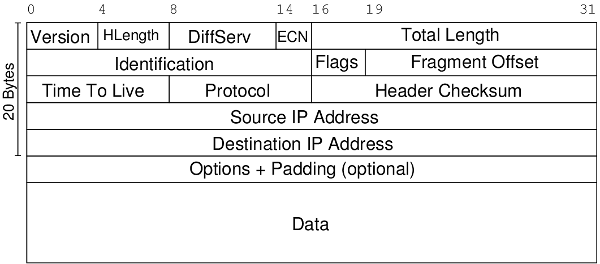
\includegraphics[scale=0.5]{ip.png}\\
Some IPs are reserved for private networks:
\begin{itemize}
\item 10.0.0.0 $\to$ 10.255.255.255
\item 192.168.1.1 $\to$ 192.168.255.255
\item 172.16.0.0 $\to$ 172.16.255.255
\end{itemize}
\textbf{Def} A \emph{datagram} is a basic transfer unit associated with a packet-switched network. The delivery, arrival time, and order of arrival need not be guaranteed by the network.\\\\
\textbf{Def} MTU maximum transmission unit\\\\
\textbf{IP fragmentation}
\emph{Identification:} 16 bit, is the unique identifier of the fragmented datagram.\\
Note that all fragments have the same identification number.\\
\emph{Flags:} 3 bits
\begin{itemize}
\item 0 Reserved, must be zero
\item DF Don't fragment\\
If set to 0 $\to$ there may be fragments\\
If set to 1 $\to$ drop datagram if it has to be fragmented
\item MF More fragments\\
0 $\to$ last fragment\\
1 $\to$ there are more fragments
\end{itemize}
\emph{Offset} 13 bits, offset of this datagram wrt the first fragment with that ID
\newpage
\textbf{Fragmentation example}\\\\
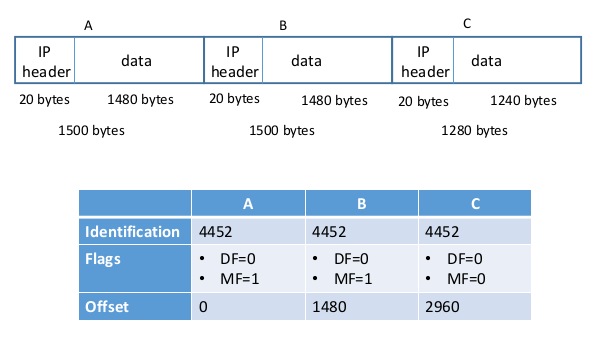
\includegraphics[scale=0.6]{fragmentation.png}\\
\begin{remark}
\textbf{DOS with IP fragments}
You keep sending fragments without sending the first fragment, the router keeps waiting for it until it exhausts its memory.
\end{remark}
\newpage
\section{ICMP} Internet control message protocol. It relies on IP and is and integral part of it.\\\\
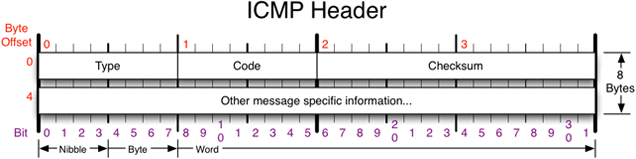
\includegraphics[scale=0.9]{icmp.png}\\\\
\textbf{Some message types}
\begin{itemize}
\item 0  Echo Reply
\item 3  Destination Unreachable\\
Code 0 $\to$ Net unreachable\\
Code 1 $\to$ Host unreachable\\
Code 2 $\to$ Protocol unreachable\\
Code 3 $\to$ Port unreachable\\
Code 4 $\to$ Fragmentation needed and DF set\\
Code 5 $\to$ Source route failed
\item 4  Source Quench
\item 5  Redirect
\item 8  Echo
\item 11  Time Exceeded\\
Code 0 $\to$ Net unreachable\\
Code 1 $\to$ Host unreachable
\item 12  Parameter Problem
\item 13  Timestamp
\item 14  Timestamp Reply
\item 15  Information Request
\item 16  Information Reply
\end{itemize}
\section{Traceroute}
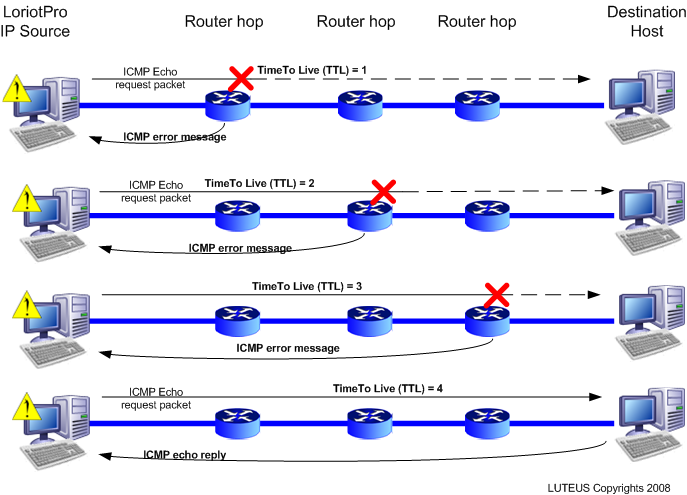
\includegraphics[scale=0.5]{traceroute.png}
\newpage
\section{Denial of service}
\textbf{Def} a Denial of Service is a type of attack that aims at congesting or overpowering a system's capacity by generating requests the system will have to answer.\\\\
\textbf{Examples}
\begin{itemize}
\item Dos with IP fragmentation
\item Ping Flooding (the attacker exploit his wider bandwidth)
\item Ping of death
\end{itemize}
\chapter{Osi Transport Layer}
\section{TCP}
The Transmission Control Protocol builds on top of IP the notion of state. Infact IP just delivers data while TCP manages the data segments by mean of checksums and re-delivery of unreceived/corrupted packets.\\
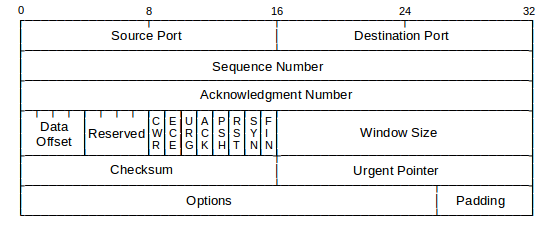
\includegraphics[scale=0.8]{tcp-header.png}\\
A server and a client that partecipate in a TCP connection open a \emph{socket} which is a tuple (source-ip:source-port,destination-ip:destionation-port).\\
Note that a client generates a source port randomly.\\
\textbf{TCP details - some flags:}
\begin{itemize}
\item \textbf{SYN:} initializes the TCP session, it should be set to 1 only for the first datagram
\item \textbf{ACK:} ackwnoledge the reception of the segment
\item \textbf{FIN:} it signals the intention of closing the connection
\item \textbf{RST:} drop the connection (reset)
\end{itemize}
\textbf{Sequence number:} it is a 32 bit generated by each end (note that the sequence number of the client is independent from the server's one).\\
\textbf{Acknoledgement number:} 32 bits\\\\
\newpage
\section{Handshakes}
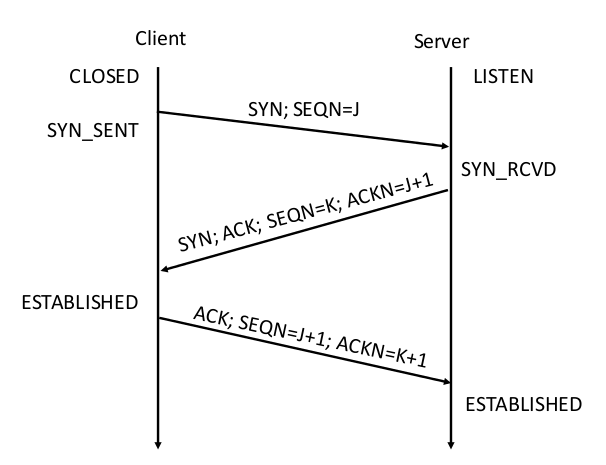
\includegraphics[scale=0.5]{3-way.png}\\\\
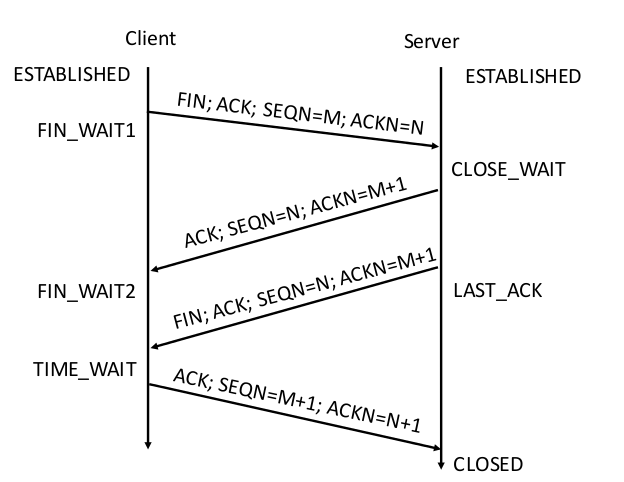
\includegraphics[scale=0.5]{4-way.png}
\newpage
\section{Some TCP specifics}
Both client and server set up a TCB (Transmission control block) to keep track of connection. The TCB structure is freed from memory when connection reaches status CLOSED.\\\\
A packet with RST flag up does not receive an answer.\\
If the state is CLOSED any packet with no RST receives a RST.\\
If the state is LISTEN 
\begin{itemize}
\item SYN flag up + no ACK opens a TCP session. Answer is SYN+ACK
\item Only ACK receives a RST
\item Drop with no answer otherwise
\end{itemize}
\section{SYN DoS}
When the server receives SYN J it answers back with SYN K, ACK J+1.\\
The server opens a new session in a separate threat/ allocates resources. Then the server waits for the ACK K+1 from the client, it waits for the MSL (maximum segment lifetime set by default to 2 minutes). The same mechanism is on the sender side but of course the attacker controls it and can bypass it.\\\\
The attacker drops all SYN ACKs with a firewall to avoid exhausting its own resources. Note that a server typically has more bandwidth than a single client.
\begin{remark}
The attack currently works in $\mathcal{O}(2n)$ because for each SYN a SYN ACK is received $\to$ less bandwidth.
\end{remark}
However the attack can be improved by spoofing the source ip address, now the attacker is operating in $\mathcal{O}(n)$.\\
In theory the attack should not work because the server should receive a RST by each zombie, consequently free the TCB making the attack fail.\\
Still the attacker can choose a set of IPs which do not reply.
\section{Dos mitigations}
\begin{itemize}
\item Load balancing: distribute traffic loads evenly
\item Rate limiter: deny traffic above a certain rate of SYN/sec
\item Proof of work: require the source to solve a cryptopuzzle before allocating resources for the connection (note that this requires a protocol support).
\end{itemize}
\newpage
\section{TCP scans}
It is possible to exploit specifications of a network protocol (TCP,UDP,..) to learn something about a system or a network.\\\\
\textbf{SYN Scan:} the attacker forges TCP packets with SYN=1. It is useful to see whether the remote system accepts incoming connections on a certain port.\\
Note that a polite way of scanning is performed in the following way: after the server's SYN ACK reply, the attacker sends a RST so that the 3-way handshake is never finished.\\\\
\textbf{Host fingerprinting:} different operating systems have their own independent implementation of the TCP stack.\\\\
\textbf{Examples:}
\begin{itemize}
\item FIN = 1
\item all flags set to 0
\item Xmas: FIN,URG,PSH = 1
\end{itemize}
\newpage
\section{TCP Session hijacking - Mitnick attack}
The attacker wants to send commands to a server they have no access to (eg. simple IP address authentication). The server has to think the attacker is the client, however the attacker does not sit in between client and server.\\\\
A TCP segment is identified and validated by:
\begin{itemize}
\item client ip $\to$ known
\item destination ip $\to$ known
\item port $\to$ known (if not standard, scan)
\item client SEQ number $\to$ known(the attacker generates it)
\item server SEQ number $\to$ \emph{unknown}
\end{itemize}
Back in the old days algorithms for generating the SEQ number were really simple.\\\\
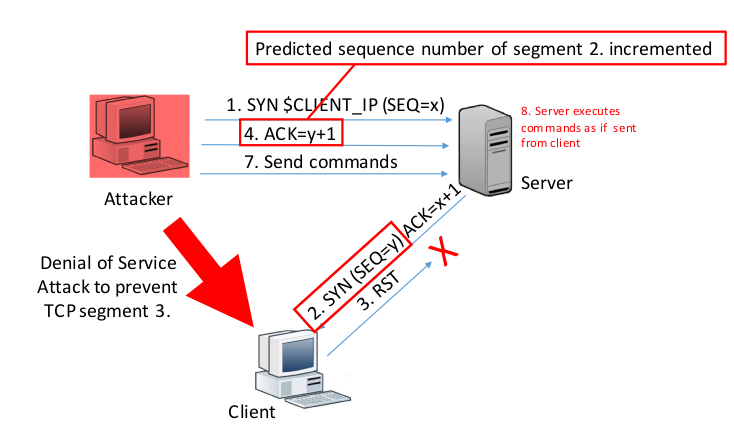
\includegraphics[scale=0.6]{mitnick-attack.png}
\newpage
\section{UDP}
The User Datagram protocol is a stateless. It is designed for fast delivery of data
\begin{itemize}
\item Data integrity can be controlloed at application level
\item It relies on the reliability of the underlying network link
\item It does not guarantee delivery (there is no ACK mechanism)
\end{itemize}
\textbf{Usage}
\begin{itemize}
\item DNS servers
\item NFS (network file systems)
\item SNMP (simple network management protocol)
\item DHCP (dinamic host configuration protocol)
\item Most real time applications
\end{itemize}
\section{UDP scans}
It can be used to discover open ports on the network:
\begin{itemize}
\item CLOSE $\to$ ICMP port unreachable
\item OPEN $\to$ no answer
\end{itemize}
However it is possible to configure a stealth system that does not reply to UDP requests to CLOSED ports by dropping ICMP packets with a firewall or router.
\chapter{Osi Session - Presentation - Application Layer}
\section{DNS}
DNS (Domain Name Service) is a hierarchical system for domain name resolving. It translates human readable addresses to IP addresses the domain is reachable at. It uses UDP for fast answer (port 53).\\
\textbf{Motivation:} it is possible to assign multiple names to the same ip or viceversa. This flexibility is useful for:
\begin{itemize}[noitemsep,nolistsep]
\item Server substitution
\item Virtual hosting (a single server hosting multiple websites)
\item A name is assigned to multiple IPs (so that the workload is distributed).
\end{itemize}
There exists different kind of DNS records, here we lista few:
\begin{itemize}[noitemsep,nolistsep]
\item \textbf{A} correspondence name - IP(s)
\item \textbf{AAAA} Same as A but works for ipv6
\item \textbf{NS} ip of the DNS server to ask
\end{itemize}
\textbf{DNS hierarchy}
\begin{itemize}[noitemsep,nolistsep]
\item Root DNSs $\to$ they are responsible for top level domain queries
\item Authoritative DNS $\to$ A DNS that "knows the answer" (ie. it does not ask to other DNSs)
\item Recursive DNS $\to$ It forwards queries to authoritative DNSs
\end{itemize}
\subsection{DNS Cache poisoning}
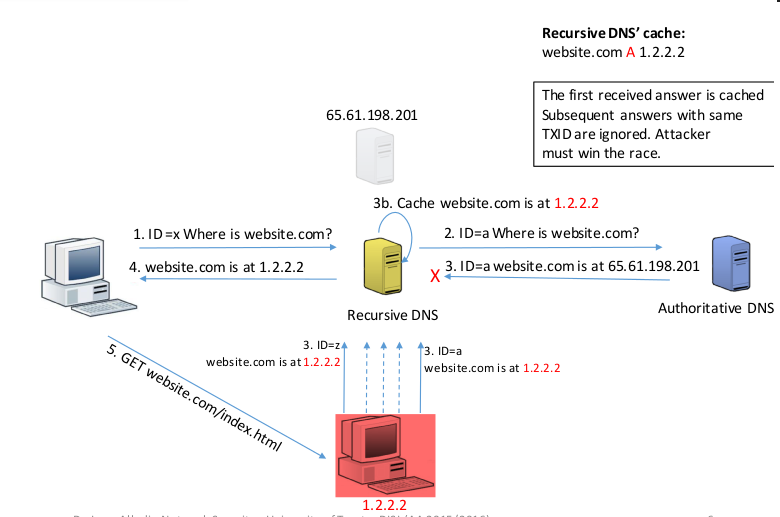
\includegraphics[scale=0.6]{dns-poisoning.png}
\newpage
\subsection{Kaminsky attack}
The attacker rather than replacing an A record replaces an NS record, in this way he can get control over any (sub)domain.\\
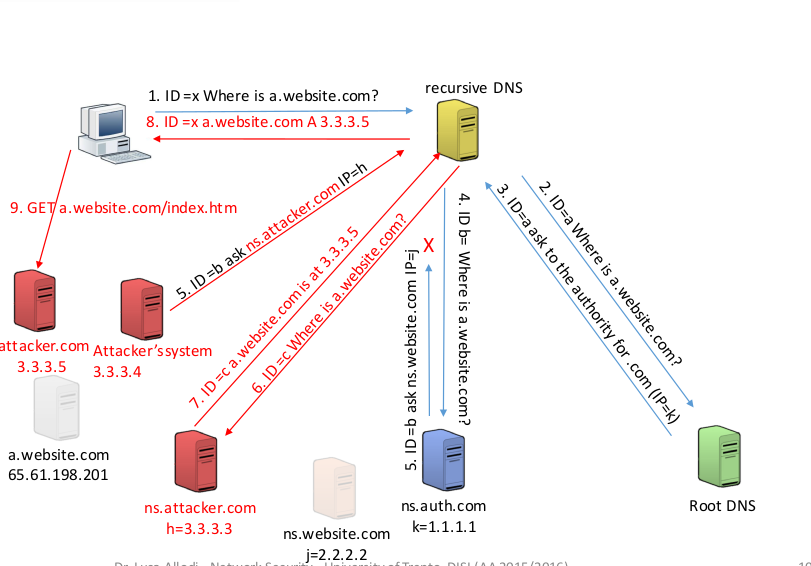
\includegraphics[scale=0.6]{kaminsky-attack.png}\\
\textbf{Mitigation:} the source of attack is low entropy with a 16 bit ID. Randomness is not enough and it is not feasible to change the protocol to 32 bits. \\
The solution is to randomize the source port to increase the entropy: any answer that does not match both source port and transaction ID will be dropped.
\newpage
\subsection{DNS amplification attack}
It is DoS attack that exploits certain types of DNS answers that are much bigger in size than the requests.\\
Recall that the DNS works over UDP so the source IP is easy to spoof.
\subsection{DNS zone transfer}
A sone is a domain for which a server is authoritative. "Slave" servers can ask "authoritative" servers to copy their zone database (over TCP).\\
An attacker pretends to be a slave server and dump the zone DB. In this way he acquires knowledge of zone's infrastructure and it is eased in performing further attacks.
\subsection{DNS Sec}
It is a secure implementation of the DNS protocol: it implements DNS auth on top of normal DNS. Note that it protects just integrity and not confidentiality.
\section{HTTP}
HTTP is the main protocol on which the www works. It is based on the notion that a client can either reuest or submit data to a server. There are two methods: GET and POST.\\
HTTP is stateless, HTTP cookies enable statefulness.
\subsection{Cookies}
\begin{itemize}
\item Domain  (who can read)
\item Expires (if NULL valid only for a session)
\item Secure (only over SSL)
\end{itemize}
\textbf{HTTP session hijacking} the attacker can read the session ID cookie and spoof the victim's identity (eg. facebook until 2011).\\
Secure cookies provide confidentiality but no integrity.
\section{Telnet}
It is a protocol used in remote control services. It operates over TCP port 23. Typically there is no authentication and no encryption.
\section{Common issues}
\begin{itemize}
\item Lack of authentication
\item Communication channel is in the clear
\end{itemize}
\chapter{Vulnerabilities}
\textbf{Software bug} a bug is a problem in the execution of the software that leads to unexpected behaviour (eg. crashes,infinite loops, wrong entries of db displayed)\\
Charachteristics of a bug
\begin{itemize}
\item Replicability
\item Logic/configuration/design/implementation
\item Fix priority
\item If it is documented it is a feature
\end{itemize}
\section{Types of vulnerabilities}
\begin{itemize}
\item Configuration v.\\
eg. Ssh accepts root connections from any ip
\item Insfrastructural v.\\
eg. sensitive db in a network's DMZ
\item Software v.\\
eg. authorization mechanism can be bypassed
\end{itemize}
\section{Vulnerability discovery}
Vulnerabilities are different in nature
\begin{itemize}
\item Often implementation dependent
\item May require deep understanding of sw module interaction
\item Necessary in-depth knowledge of system design (kernel structure, memory allocation)
\end{itemize}
Discovery techniques
\begin{itemize}
\item Code lookups (searches for known patterns)\\
either you are a developer or the software is open source
\item Fuzzing (semi-automatic random input generation)
\item Google hacking (outdated)\\
you look for software that you already know it is vulnerable
\end{itemize}
Vulnerabilites can be found either internally or externally to a company.\\
\section{Vulnerability handling}
The ISO 30111 is a standard to handle vulnerabilities.\\
\textbf{The initial investigation}
\begin{itemize}
\item The reported problem is a security vulnerability
\item The vulnerability affects a supported version of the software the vendors maintains, not third parties modules (else: exit).
\item The vulnerability is eploitable with know techniwues (else: exit)
\item Root cause analysis
\item Prioritisation (evaluate potential threat)
\end{itemize}
\textbf{Resolution decision}\\
Vendor must decide how to resolve the vulnerability.
\begin{itemize}
\item Configuration v. $\to$ advisory may be enough
\item Code v. $\to$ patch
\item Critical v. $\to$ release a mitigation before full patch
\end{itemize}
\textbf{Remediation development}\\
Every solution must be tested before being delivered. This is very expensive both for customer and vendor\\\\
\textbf{Release and Post-Release}\\
\section{Different issues}
Vulnerability advisories are typically published after pathcing.\\
Security researchers expect economic return and or credit.\\
Issue: communication between security researcher and the vendor: tradeoff between saying little and being verbose.\\
Often involves development of Proof of concept exploit to show the vulnerability is exploitable.
\section{Social Engineering}
\textit{The biggest threat to the security of a company is 
not a computer virus, an unpatched hole in a key 
program or a badly installed firewall. In fact, the 
biggest threat could be you. What I found personally 
to be true was that it's easier to manipulate  people 
rather than technology. Most of the time 
organisations overlook that human element}\\
Kevin Mitnick\\\\
Social engineering identifies a set of techniques that attack weaknesses in human psychology.\\
Situational theory of publics: why people take action, or feel part of a collective
\begin{itemize}
\item Problem recognition $\to$ subject thinks the problem is relevant to them
\item Active involvement $\to$ subject thinks he will suffer the consequences of the threat
\item Constraint recognition $\to$ subject thinks his actions are limited by factors outside of their control
\end{itemize}
\subsection{ELM - Elaboration Likelihood Model}
ELM describes the ways humans change their attitudes or decide to perform actions they would not perform without external "stimuli".\\
Two routes to persuasions:
\begin{itemize}
\item Central route\\
Stimuli are weighted by the subject and the final decision is carefully elaborated. Persuasions happens through careful elaboration of information
\item Peripheral route\\
Subject is convinced by under analyzing apparently relevant clues that are in reality unrelated to the subject matter. Examples of adjunct elements of the communication: likeability of subject,attractiveness,trust,etc.
\end{itemize}
\begin{remark}
Social engineering differs from marketing in that attackers typically do not try to sell products. Rather social engineers must persuade victims to disclose sensitive or private network.
\end{remark}
\subsection{Hacking a human}
\begin{itemize}
\item \textbf{Reciprocation}\\
Normative Commitment: subject will perform an action because it is customary or mandated by law or contract. It is based on the notion of reciprocation of benefits. When subject receives something he values he feels \emph{cognitive dissonance} (eg. sun cream free tester example). People tend to comply because they feel gratitude for the unsolicited proposal.
\item \textbf{Consistency}\\
Continuance commitment: subject keeps doing a determined actio even if it is clearly bad (eg. lottery, keep spending money, eventually it will work).\\
Upfront costs are low wrt promised benefit.
\item \textbf{Social proof}\\
Affective commitment: people are influenced by the opinion of those they esteem or like. Example: pretend you are on a vacation with a friend of the victim and ask money to solve an emergency
\item \textbf{Likeability}\\
If you like somebody you will trust him and viceversa\\
Example: actors in advertisment
\item \textbf{Authority}\\
Subjects fear punishment and will comply\\
Example: Milgram's experiment with electric shocks
\item \textbf{Scarcity}\\
Subject think freedom of choice is a function of time: similarly to fear scarcity leads people to take quick potentially uninformed decisions in fear of losing an opprtunity that will disappear in time or scarce in quantity. 
\end{itemize}
\chapter{CVSS}
Why to grade vulnerability?\\
Vulnerability counting can not be a measure of severity. Vulnerabilities are not the same (eg. XSS vs BoF). Clients and user should be informed too: security researcher $\to$ vendor $\to$ user. A standard is needed.\\\\
CVSS is an open framework for communication the characteristics and severity of sw vulnerability. The goal is different users score the same vulnerability in the same way $\to$ severity assessment and different people read the same vulnerability in the same way $\to$ severity communication.\\
\begin{remark}
CVSS v2 and v3 are different
\end{remark}
CVSS v3 has three metrics:
\begin{itemize}
\item \textbf{Base metric}\\
Exploitability metrics: attack vector, attack complexity, privilegs required, user interaction\\
Scope metric (where is the vulnerability and wrt whom is affected)\\
Impact metrics (CIA)
\item \textbf{Temporal metric}\\
Exploitability, remediation level,report confidence
\item \textbf{Environmental metric}\\
CIA requirements,mitigated base metrics
\end{itemize}
\textbf{Example:} think of ssh open to the wild or available just in the LAN, the environmental metrics measures this difference.\\
\chapter{Malware}
\textbf{Def} a software that urn without consciousness of user and or system.\\
Two different kinds: program that need a host program to operate and self-independent ones. Moreover a malware can self replicate or not.
\textbf{Taxonomy}
\begin{itemize}
\item Virus $\to$ modifies legitimate software
\item Worm $\to$ self-replicates
\item Trojan horse $\to$ allows remote control of machine
\item Keyloggers $\to$ send typed info to attacker
\item Rootkit $\to$ hook to libraries or system files
\item Zombie,bot $\to$ remote coordinated control of multiple machines
\end{itemize}
\section{Virus}
Software that replicate and install itself without user consent. The copies can be installed into programs,data files,boot sector,macro files.\\
Components:
\begin{itemize}
\item Infection mechanism: enables replication
\item Trigger: event that makes payload active
\item Payload: (malicious or benign)
\end{itemize}
The executable changes in size so the virus is easy to spot with a hash table.\\
However the virus could place itself in an used PE header so there is no change in size.\\
\textbf{Concealment mechanism}
\begin{itemize}
\item Encrypted virus
\item Polymorphic virus
\item Metamorphic virus
\end{itemize}
A virus can modifiy the MBR so it is loaded in memory even before the operating system.
\section{Rootkit}
The kernel is organized in protection rings. Eg. going from inside to the outside: hardware,drivers,application,user space.\\
The rootkit can inject to kernel and defeat disk encryption eg. stone bootkit.\\
It can be persistent or memory based, in user level or kernel mode.
\section{Counter measures}
Prevention is ideal but difficult. Realistically you need: detection,identification,removal. Virus and antivurs tech have both evolved:
\begin{itemize}
\item Signature scanners\\
Every time the malware is loaded in memory it will look the same\\
It is a purely reactive strategy $\to$ unknown malware does not have a signature
\item Heuristics: checks for common features\\
Instead of having a perfect match it uses common features.
\item Identify actions: behavioral fingerprint
\item Machine learning
\end{itemize}
Evolution against heuristics $\to$ polymorphic virus\\
It changes how it looks in memory through encryption for every new instance.\\
Defense $\to$ generic decryption (aka sandboxing).\\
At execution time code will be the same, at that point signature and heuristics work. Still malware can recognize if it is executed in an emulated environment, if so it will not decrypt its payload.\\
Evolution $\to$ metamorphic virus: they rewrite the machine code in an automatic way. Fortunately this is very difficult to perform (eg. 14.000 lines of assembly code)\\
Defense $\to$ behavioural detection: the basic idea is that malware behaves differently from legitimate software (eg. system calls, interaction with drivers, system interrupts). The risk of false positives is higher compared to signature and heuristics (for which an hash collision is needed).
\newpage
\section{Botnets}
\textbf{Def.} a botnet is a virtual network of infected machines under the control of a "bot herder".\\
It is managed through a command and control server which can push configuration files and update functionalities.
\subsection{Centralised archtecture}
Bots communicate with the bot herder via IRC or HTTP. For the latter there a re two approaches: either the bot contact a fixed (set of) IP or it resolves domain dynamically.\\
C\& C server is a single point of failure: who controls the C\&C controls the botnet.\\
Centralised botnets take downs happen by \emph{sinkholing}: C\&C server needs to be protected:\\\\
\textbf{Fast-flux:} one domain is mapped to different IP addresses\\\\
\textbf{Domain-flux:} each bot generates valid domain names periodically with a DGA (domain generation algorithm) and resolves them. If bots get no answer from a generated domain they pass to the next in the list. If the DGA generates a domain which already exist then botnets may cause an unintentional dos attack.
\subsection{P2P architecture}
It is more robust than centralised. Commands are spread through the network, bots can act as both slaves and masters. When a new machine is infected:
\begin{itemize}
\item Hard coded list of peer are contacted
\item Mixed p2p/centralised approach (eg. a centralised web cachce with list of peers)
\item Infected bot inherits peer list from infector
\end{itemize}
There are three types of p2p botnets:
\begin{itemize}
\item \textbf{Parasite}\\
All bots are selected from vulnerable hosts within an existing p2p network
\item \textbf{Leeching}\\
Bot candidates may be vulnerable hosts that were either inside or outside an existing p2p network.
\item \textbf{Bot-only}\\
It builds its own network in which all members are bots.
\end{itemize}
\textbf{Usage:} botnets are used to perform DDoS,send spam,exploit computational power, steal sensitive information, be rented to other criminals.
\chapter{Web attacks}
\textbf{Attacker's evolution}\\
In the 90's attackers were security enthusaistics with high technical competence. In the 00's attackers were mainly script kiddies running automated tools while in '10s attackers are economic agents: malware is an investment.\\
A malware author operates in a competitive and adversarial envrironment:
\begin{itemize}
\item Adversaries: security researchers,security firms building AV signatures for malwares
\item Competitors: many players in the market and a finite number of vulnerable systems.
\end{itemize}
\section{Propagation vs operation}
Different strategies:
\begin{itemize}
\item High propagation rate (self-replication) $\to$  higher chances to handle a sample to security researcher
\item Low propagation rate (controlled deployment) $\to$ higher stealthiness
\end{itemize}
There is an equilibrium point whereby all competing players maximize their expectations in terms of return to investment.\\
\section{Malware distribution network}
Moder internet malware does not employ self propagation mechanism (worms are not of concern anymore).\\
Nowadays the attacker deploys the malware on a machine he controls, the infected machines contact the malware server.\\
Sources of risk
\begin{itemize}
\item Domain compromisation
\item Content compromisation (eg. XSS)\\
Execution can be upon page loading, events triggering, user actions.
\item Malicious third party
\end{itemize}
\textbf{Drive by downloads:} it is a common infection mechanism. when contacted the server delivers content that tries to exploit local vulnerabilities on the machine (eg. bufer overflow against the browser or browser plugins). If successful shellcode calls home, downloads malware and executes it.\\\\
\textbf{third party traffic:} an attacker buys connections from specific users with specific configurations (eg. js check local configuration,sends it to remote server, the user loads the webpage the attacker compromised and if characteristics match traffic is redirected.
\section{Exploit kits}
Exploits typically attack vulnerabilities on adobe flash, acrobat reader, IE, Java, plugins etc.\\
\textbf{Offensive components}
\begin{itemize}
\item Detect browser and operating system
\item Check wheter the system has been already attacked by ip checking as a cookie is not so stealthy and moreover cookies can not be retrieved from new domains.\\ This is a business model, it wants to keep a low profile under the radar
\item Check if the sytem is vulnerable
\item It launches appropriate attack
\end{itemize}
\textbf{Defensive components}
\begin{itemize}
\item Many exploit kits defend themselves against AV/robot detection
\item Payload and malware obfuscation
\item Block ip to avoid probes
\item Evasion robots+ crawlers
\item Some even check whether the domain on which the exploit kit is hosted is included in antimalware list.
\end{itemize}
\chapter{Advanced DoS}
\begin{itemize}
\item Reflected DoS A reflector is a server that will reply to any receiving packet. Nowadays you would need a lot of bots to saturate all the bandwidth. instead of infecting million of bots you build a list of reflector that the slaves can contact. It is a classic IP spoofing scenario.
\item Amplification DoS
Eg. Network Time Protocol
\end{itemize}
\section{Mitigations}
\begin{itemize}
\item Source identifications\\
It is a kind of traceback. It is quite difficult
\item Capabilities\\
Capability is made of marks (unique hash values) set by routers on the path from sender to receiver. Routers check validity of marks upon response.
\end{itemize}
\textbf{Capabilities limitation:} capability can be saturated
\chapter{Cyber crime market}
There can be many type of markets: financial,work/job position etc. \\
Cyber markets were originally in IRC (but being unorganized it failed completely) and then moved to web-forums. What is traded? Data,knowledge and services: eg. attacking tools, exploits, vulnerabilitites,accounts,money laundry,CCNs etc.
There are two kind of market:
\begin{itemize}
\item TOR based market\\
It is mostly on illegal goods in traditional sense (eg. drugs,weapons)
\item Closed market
\end{itemize}
These markets are closed by entry selection. Some of them are typically national: eg. russian,chinese. Note that this "authentication" mechanism based on the difficulty of learning the language is not secure.\\
Markets can offer low-tech services (spam advertize,stolen credentials) or high tech: attack delivery technologies,malware/specialized payloads.
\section{Composition of an attack}
Elements of an attack
\begin{itemize}
\item User connections
\item Attack delivery
\item Malware infection
\item Monetisation mechanism
\end{itemize}
Most products sold in the markets enable the attacker to perform only one of these steps:
\begin{itemize}
\item Traffic brokers,stolen accounts $\to$ connections
\item Exploit kits,stand alone expoloits $\to$ attack delivery
\item Ransomware,banking malware $\to$ malware
\item CCn,banking info $\to$ monetisation
\end{itemize}
Each of these steps can be combined by an attacker to obtain a set of characteristics that suits them
\begin{itemize}
\item Traffic from northern europe
\item Exploit kits for recent IE versions
\item Malware that does not infect CSI countries
\item Attack UK bank costumers
\end{itemize}
\chapter{System hardening}
All the system have a default configuration (pc,servers,mainframes). Moreover fresh installations of an operating system offer default services (DHCP,NetBios,SSH,VNC).\\
System hardening is the process by which a system's configuration is tuned to improve its security without compromising its functionality.
\section{Attack surfaces}
\begin{itemize}[noitemsep]
\item Weak passwords
\item SW vulnerabilities
\item Misconfigurations
\item Services listening on the network
\item Inaccurate access control
\end{itemize}
\textbf{Minimality principle:} no user and no system component or process should be authorised to perform actions that are not strictly necessary for their normal operations.\\
It can be applied to both users and processes.\\
A \emph{system} should be configured such that it does not embed or enable functionalities that are not needed for normal operation (eg. microkernel)\\
A \emph{user} should be authorised to only access and modify resources that are necessary for their normal operations.\\
\textbf{Example:} compile the kernel with just what is needed.
\section{User authentication}
There are two steps: \emph{identification} and \emph{verification}. The final goal is to link the physical user with its representation in the system. Here we list four means of authentication:
\begin{itemize}[noitemsep,nolistsep]
\item Knows: password,PIN,graphical password
\item Posses: key,token,smartcard
\item Is (static biometric): fingerprint,retina
\item Does (dynamic biometrics): voice,sign
\end{itemize}
They can be used alone or combined and of course they all have problems.
\subsection{Knows}
\textbf{Password aging}
"Frequently" change passwords decreases attack surfaces (less time for attacker to crack hash file). However users will have to create and remember more passwords for one account. It is important to give users time to think of good password (eg. do not force users to change the password before they can log in). There must be a balance between security and usability.\\\\
\textbf{Draw a secret scheme}\\
It is easier to remember and there are low error rates but still adjacent coordinates are more likely to be used in sequence.\\\\
\textbf{Graphical password}\\
The user clicks on some pixels among a set of highlighted ones and then to log in the users will have to click (possibly in the same sequence). Drawbacks: shoulder surfing; is it easy for the user to change?
\subsection{Posses}
\textbf{Token authentication}\\
Examples: magnetic stripe card,memory card,smartcard etc.\\
Token based: it is used to compute a response to challenge. It can be used to prevent shoulder surfing (even if the attacker sees the current value he can not predict the next valid one).\\
The most common challenge-response mechanism is based on time syncronization: token and server have a syncronized clock so they will generate the same number at a given time.\\\\
\textbf{Memory card}\\
It stores but it does not process data. It easy to read and replicate the magnetic strip.\\\\
\textbf{Smartcard}\\
They have their own processor,memory,I/O ports. They include a crypto chip, they are tamper resistant.
\subsection{Biometric}
\textbf{Physiological (static):} iris,fingerprint, hand,retinal and face recognition\\
See picture for graph/accuracy: 
\begin{itemize}
\item Hand $\to$ sweat palms, temperature
\item Face $\to$ glasses,beard,light conditions,picture of a face,make up etc.
\item Voice $\to$ cold
\end{itemize}
\textbf{Behavioural (dynamic):} voice,typing pattern,hand signature,gesture,gait.
\chapter{Firewall}
Firewalls are perimetral network components that filter incoming (outgoing) traffic from (to) the network.They have different policies:\\
\textbf{Default deny:} nothing is allowed to pass expect what is permitted\\\\
\textbf{Default permit:}everything is allowed except for what is denied\\
It is suitable for open organizations like universities or home systems.\\\\
\textbf{Firewall types:}
\begin{itemize}
\item Static packet filtering
\item Stateful packet filtering
\item Proxies (application-level or circuit level gateways)
\end{itemize}
\textbf{Firewall basing}
\begin{itemize}
\item Stand alone machine
\item SW module in router or LAN switch
\item Bastion host
\item Host-based firewall (see slide)
\item Personal firewall (see slide)
\end{itemize}
\newpage
\section{Static packet filtering}
Header information is used for filtering (eg. protocol number,source and destination ip and port numbers). Stateless: each IP packet is examined isolated from what is happened in the past. \\
It is often implemented by routers, it is simple and fast and has a low demand on resources.
\textbf{Access lists}\\
\textbf{Standard ACL:} \$ number \$ action \$ src (wildcard)	
\begin{itemize}
\item Number $\to$ identifies rule
\item Action $\to$ accept/deny
\item Src $\to$ source ip
\item Wild card (inverse of subnet mask) $\to$ it says which part of the IP should be checked
\end{itemize}
\section{Stateful packet filtering}
It looks at the history of the packets passing through the firewall.\\
Stateful firewalls allow user to define states over stateless protocols. For these protocols there is no termination sequence (eg. TCP FIN 4-way handshake) so a timeout is implemented, depending on the application.\\
Possible states
\begin{itemize}
\item NEW $\to$ packet trying to open a new connection
\item ESTABLISHED $\to$ incoming packet is realtive to a connection already initiated
\item RELATED $\to$ new connection related to an existing one (eg. FTP)
\item INVALID $\to$ none of the above (eg. incoming packet with ACK  but not belonging to EASTABLISHED connection)
\end{itemize}
With a stateful firewall you can prevent ACK scans (OS fingerprinting).\\
\textbf{Pros:} more powerful rules, policy definition is much simpler, very diffused.\\
\textbf{Cons:} severe impact on firewall performance, deep packet inspection slows down packet check, application support may be very complicated.
\newpage
\section{Network topologies}
\emph{If you want a firewall to work you have to put it in the right place}
\subsection{Simple configuration}
Border router implementsstatic inward and outward filtering. The best policy is to drop packets with no answer. Eg. do not allow packets whose final destination is the firewall.  The firewall has several inward facing network interfaces. Each interface is dedicated to a network level. It is a single point of failure.\\
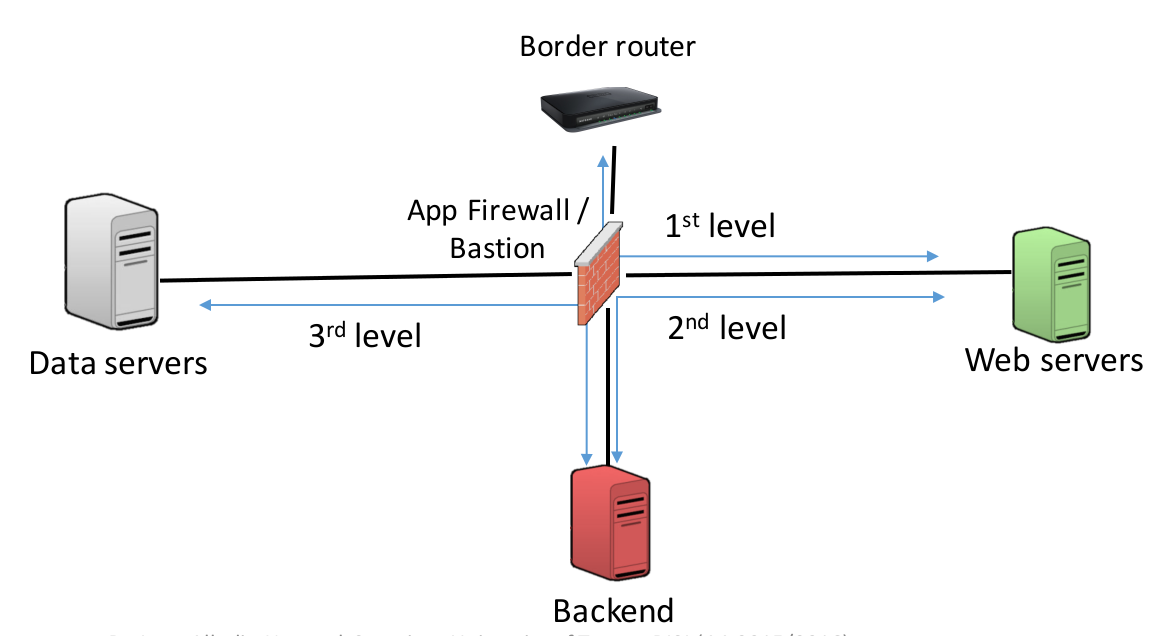
\includegraphics[scale=0.3]{firewall/simple.png}
\subsection{Divide et impera: cascade}
Interdependent firewall policies. Eg. firewall at level 1 must allow packets eventually directed toward level 2. It requires a good mixture of NAT and PAT policies,firewall configurations and good separation of services. It has high design, management and mainteinance costs.
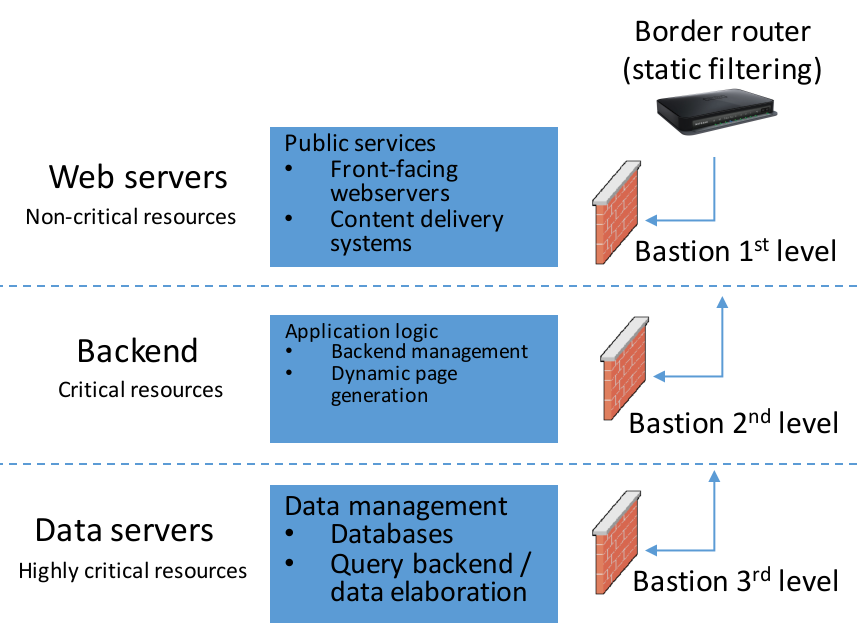
\includegraphics[scale=0.3]{firewall/cascade.png}
\subsection{Divide et impera: parallel}
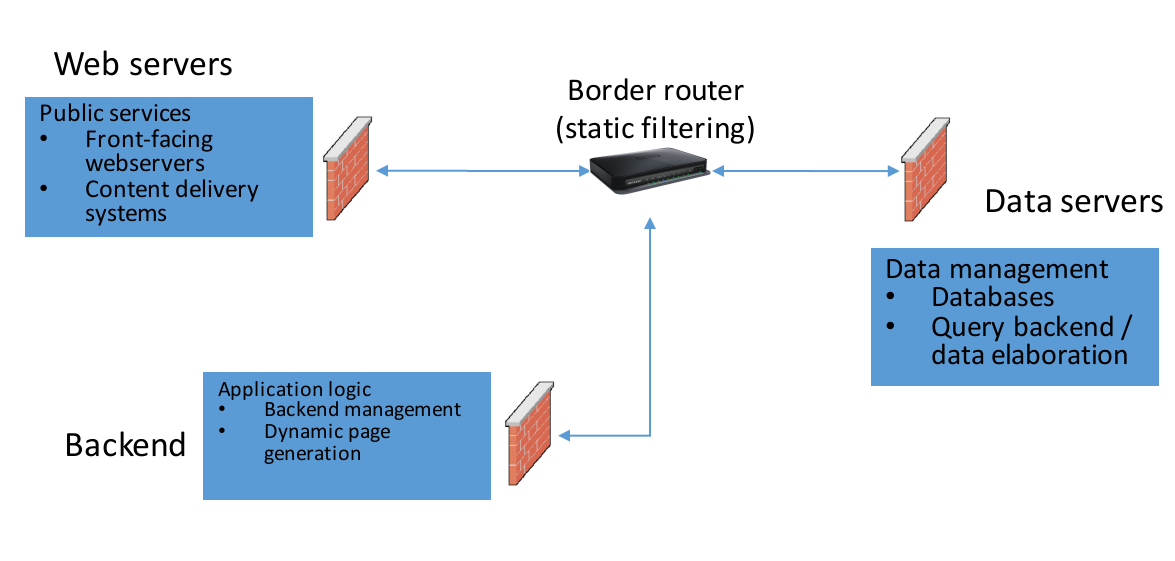
\includegraphics[scale=0.3]{firewall/parallel.png}
\subsection{Mixed}
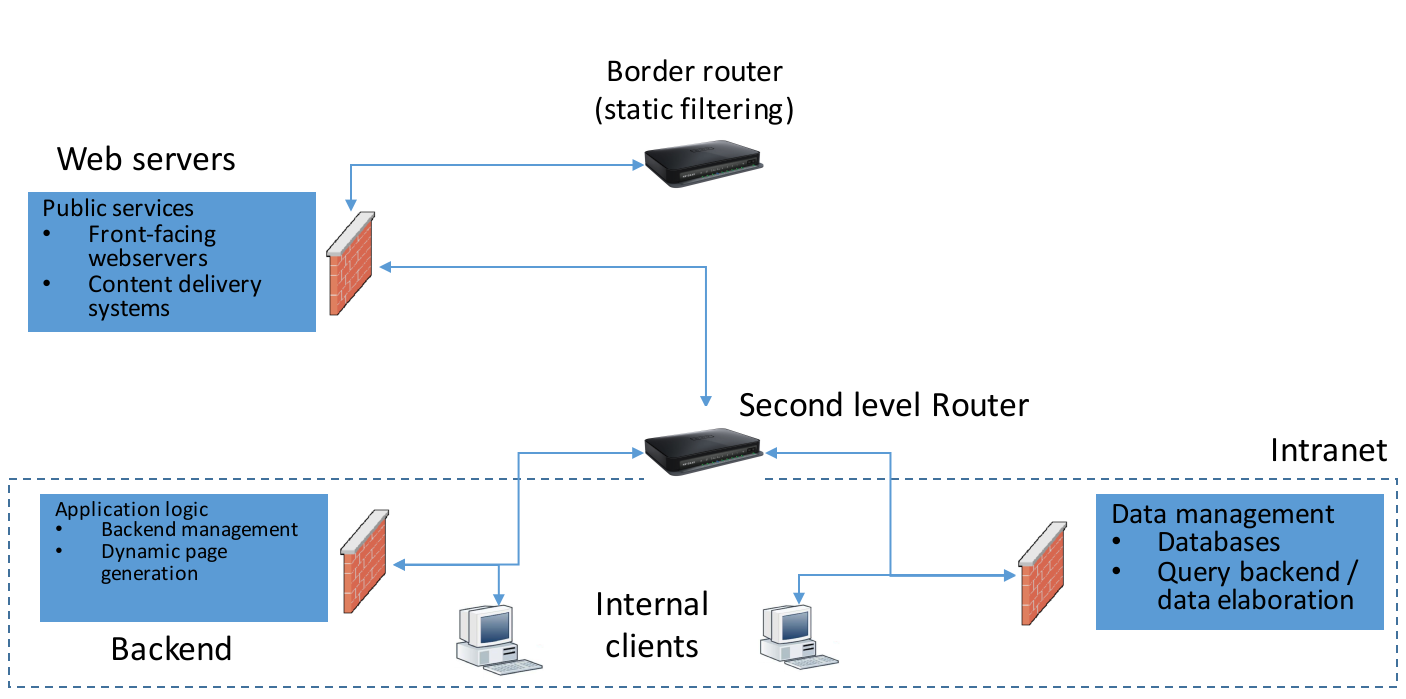
\includegraphics[scale=0.3]{firewall/mixed.png}
\section{Proxy}
\textbf{Def.} It is a network component that mediates network communications.\\
Proxy acts both as a client and server.
\subsection{Open proxy}
Proxy connnects any client on the internet to any server on the internet.\\
It enables the user to achieve some level of anonymity on the network. Note that there are techniques that allow the server to know the client's ip thorugh third parties (eg. flash). \\
Trust issues $\to$ all trust is put on proxy service (it is ok to bypass organisation's blacklist) but probably not trustworthy for sensible internet traffic. It may also be sued for malware distribution.
\subsection{Reverse proxy}
The situation is "double blind": the client thinks he is talking to the (lets say) FTP server but actually he is talking to the reverse proxy.\\
\textbf{Pros:} hide properties of internal servers (IP, non custom service ports, versioning - if too aggressive it may cause disservice eg. declaring a fake server version breaking the protocol). It may be used for load balancing (several internal replicas of a webserver) or caching server's content.
\subsection{Application level proxy}
\textbf{Pros.} information hiding, robuts authentication and logging, cost effective,less complex\\
\textbf{Cons.} keeping up with new applications, custom implementations may be expensive.
\subsection{Circuit level proxy (or gateway)}
It operates at level 4 on OSI scale. It simply crosses client connection to inside hosts.
\subsection{Network address translation}
NAT operates at level 3 and acts as a reverse proxy. It maps (sourceIP, sourcePort) to (destIP,destPort). Port address translation (PAT) to resolve conflicts.
\section{Bastion host}
It is a system identified by the firewall administrator as a critical strong point in the network security.
\begin{itemize}
\item Secure version of OS (hardened system)
\item Only essential services
\item Each proxy maintains detail audit information
\item Each proxy runs as a non-privileged separate user
\end{itemize}
\section{Administration}
\begin{itemize}
\item Access with secure connecion
\item Logging: on a remote logging server
\item Strategies of disaster recovery
\item Security incidents
\end{itemize}
\chapter{Intrusion detection system}
There are three phases
\begin{itemize}
\item Data collection\\
It can be host based or network based
\item Data analysis\\
Two distinct approaches: misuse detection ( list unwanted behaviour) or anomaly detection (build an average profile, report if current activity is significantly different from average)
\item Action\\
Report, log entry and (just IPS) block/alert
\end{itemize}
\textbf{Misuse detection}\\
It is the IDS equivalent of "default allow" policies. There are "blacklist" patterns that are believed to be related to malicious activities (eg. system calls and payloads in network protocol). It is signature based and it can only detect patterns that are already known.\\\\
\textbf{Anomaly detection}\\
It assumes intruder behaviour differs form legitimate profile. Problem: users evolve: a new legitimate activity may look suspicious.
\section{Architectural aspects}
\textbf{External NIDS}
\begin{itemize}[noitemsep,nolistsep]
\item Analysis of all incoming traffic
\item Only general signatures 
\item All "detected attacks" are logged
\end{itemize}
\textbf{Internal NIDS}
\begin{itemize}[noitemsep,nolistsep]
\item Analysis only of traffic allowed by the firewall
\item More specific signatures are possible
\item It says nothing about attacks attempted but blocked by the firewall
\end{itemize}
\newpage
\section{NIDS evasion}
Signature based evasion can be fairly trivial: for instance $"/bin/bash"$ will be detected while $"/etc/../bin/bash"$ will not. This is a proof of concept: of course NIDS could use regexp or wildcard. More advanced techniques are typically based on IP fragmentation.
\subsection{Reassembly time-out}
The NID will wait for a shorter (compared to the client) amount of time for the second fragment.
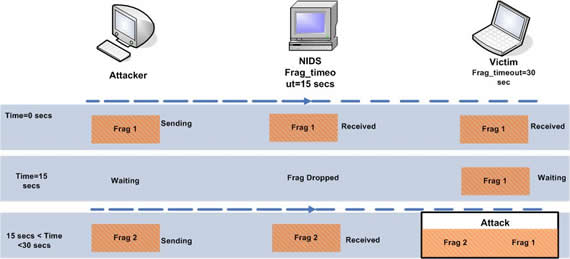
\includegraphics{IDS-evasion/1.jpg}\\
Viceversa NIDS has higher riassembly timeout than receiving client\\
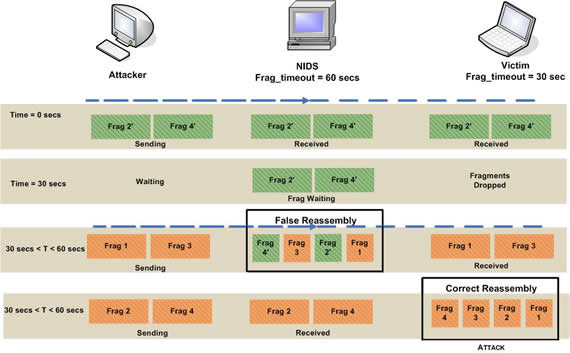
\includegraphics{IDS-evasion/2.jpg}
\subsection{Time to live}
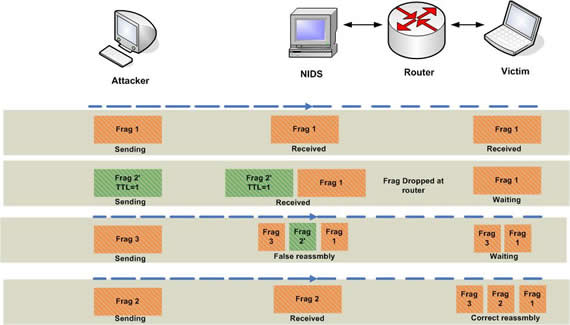
\includegraphics{IDS-evasion/3.jpg}
\subsection{Fragment replacement}
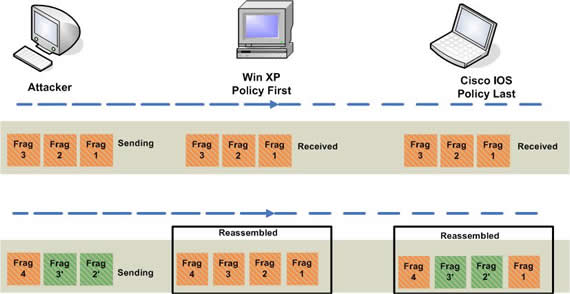
\includegraphics{IDS-evasion/4.jpg}
\chapter{Vulnerability mitigation}
\section{OS vulnerability mitigation}
\textbf{DEP:} Data execution protection - data in memory is marked as non executable. It defeats code execution via stack corruption. Still with DEP attacker can redirect execution of code areas in memory. Eg. write a stack frame in memory and point to libc. Most memory corruption attacks rely on the attacker being able to guess start address of stack frame/heap/other areas of memory.\\
\textbf{ASLR:} address space layout randomization - it randomizes location in memory of stack, heap and libraries.
\section{Vulnerability patching}
Problems related to patches: 
\begin{itemize}
\item Reboot is often required
\item SW functionalities may change
\item Deprecated third-party libraries
\item Production systems need to be up and running
\item A patch needs to be tested
\end{itemize}
\begin{remark}
Counting vulnerabilities $\neq$ Security assessment. More vulnerabilites do not translate directly into risk of attacks. CVSS measures severity NOT risk.
\end{remark}
\section{CVSS vs Exploitation levels}
\begin{itemize}
\item EL1: $\exists$ vulnerability 
\item EL2: $\exists$ PoC 
\item EL3: the exploit is traded
\item EL4: the vulnerability is reported and exploited
\item EL5: real measure of the frequency of exploitation
\end{itemize}
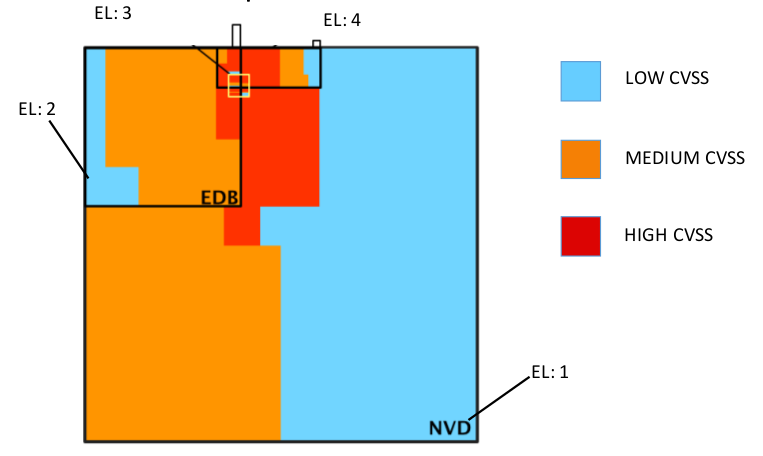
\includegraphics[scale=0.5]{comparison.png}
\end{document}